\section{Vistas}

Pasaremos a ahora a presentar los distintos diagramas para continuar modelizando nuestro problema.\\


En una primera instancia presentaremos el diagrama de clases, acompañado de sus predicados de OCL. 

Como dijimos anteriormente, presentaremos nuestra solución dividiendola en 3 etapas: Preparación, sufragio y conteo. 

Contamos con 5 tipos de diagramas, analicemos un poco las ventajas y desventajas de cada uno antes de comenzar.

\paragraph{Diagrama de contexto} 

El diagrama de contexto es una de las piedras angulares de este trabajo, nos permite observar las interacciones entre agentes. A su vez, no tenemos orden de las acciones ni una relación temporal lo cual nos impide modelizar muchas situaciones.

\paragraph{Diagrama de clases y OCL}

El diagrama de clases nos presenta una visión general de lo que vamos a modelizar, a su vez nos define un poco más las relaciones entre las clases de nuestro sistema. Permite dar una panorama general de como se comportan las clase entre ellas y que se le atribuye a cada una. Al mismo tiempo, el diagrama no permite expresar todo, para esto usaremos OCL, un lenguaje que expande al diagrama y nos permite expresar más relaciones entre clases.

\paragraph{Diagrama de casos de uso}

Este diagrama nos permite describir la interacción entre el sistema y los distintos actores 
externos. Junto a la descripción de los casos de uso, construye un detalle importante para la 
construcción del sistema.

\paragraph{Diagrama de Actividad}

El diagrama de actividad pone un orden relativo en los casos de uso. Y los relaciona aún más con los actores.

\paragraph{Máquinas de estado finitas}

La máquina de estados permite la composición entre varios actores con el mismo comportamiento y a su vez nos permite dar un orden temporal de los eventos. \\


Presentaremos primero el diagra de contexto y el diagrama de clases.


\newpage
\subsection{Diagrama de Contexto}

\begin{figure}[h!]
\centering
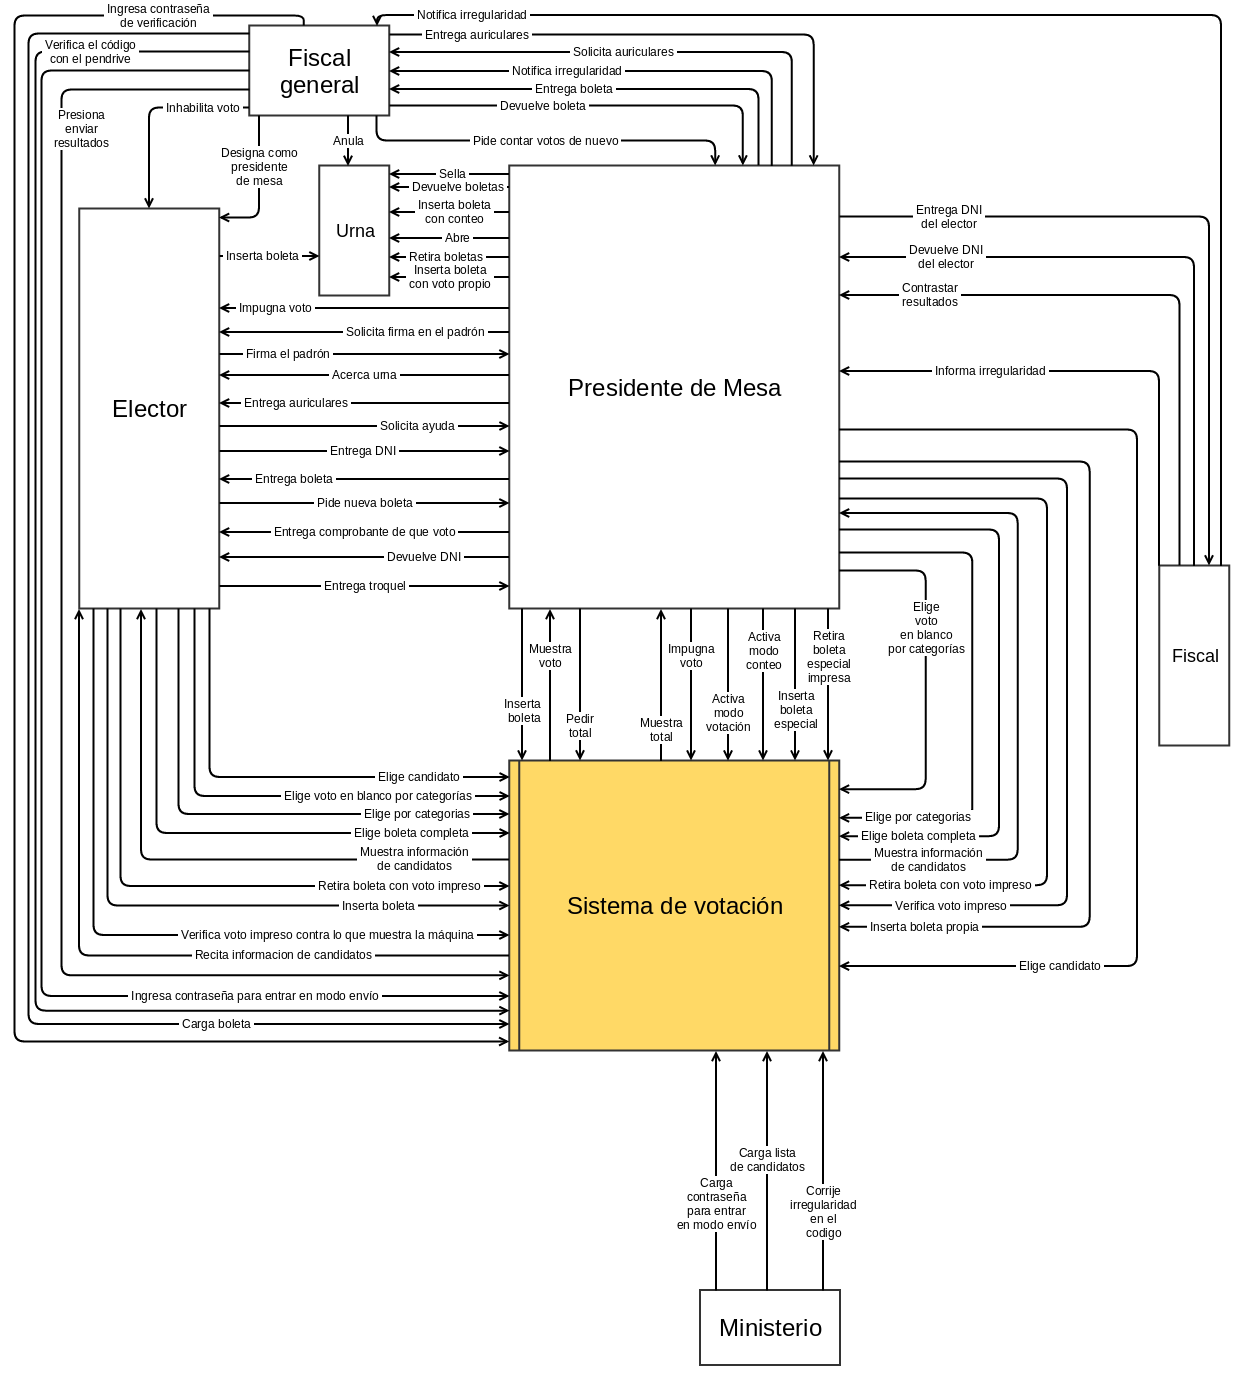
\includegraphics[scale=0.36]{imagenes/contexto1}
%\captionof{figure}{Diagrama de actividad}
\end{figure}

\newpage

\begin{figure}[h!]
\centering
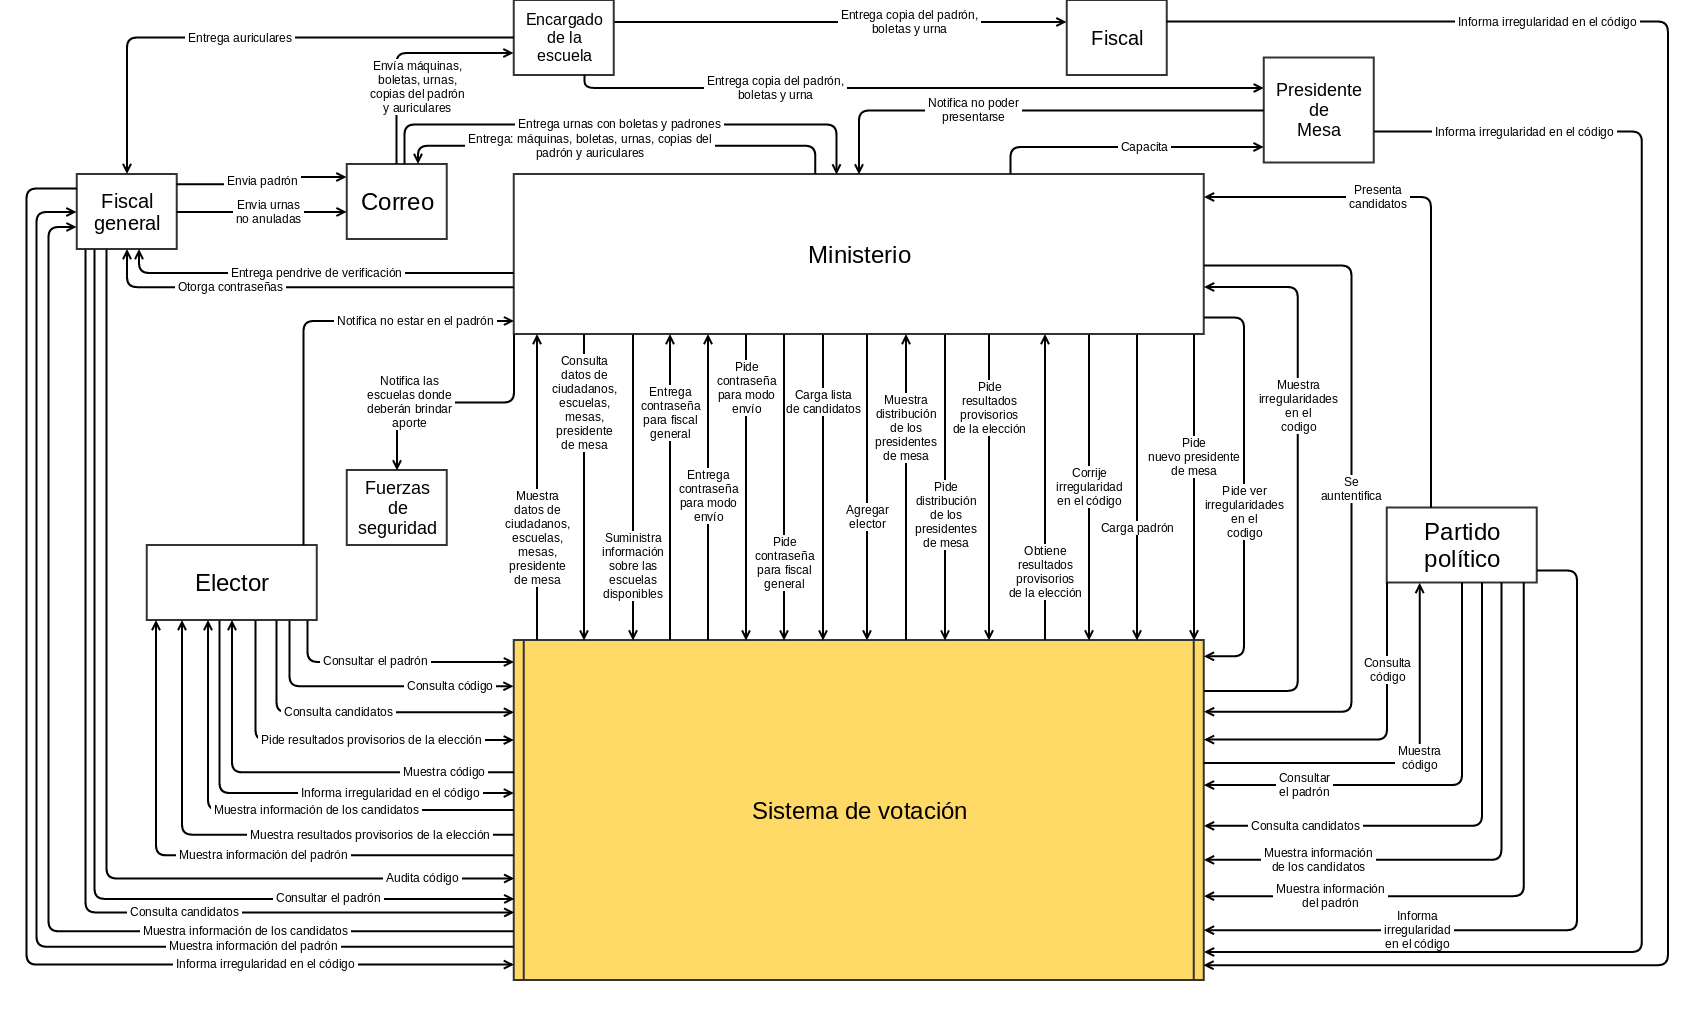
\includegraphics[scale=0.28]{imagenes/contexto2}
%\captionof{figure}{Diagrama de actividad}
\end{figure}

\newpage
\subsection{Modelo Conceptual}

\begin{figure}
  \begin{center}
	%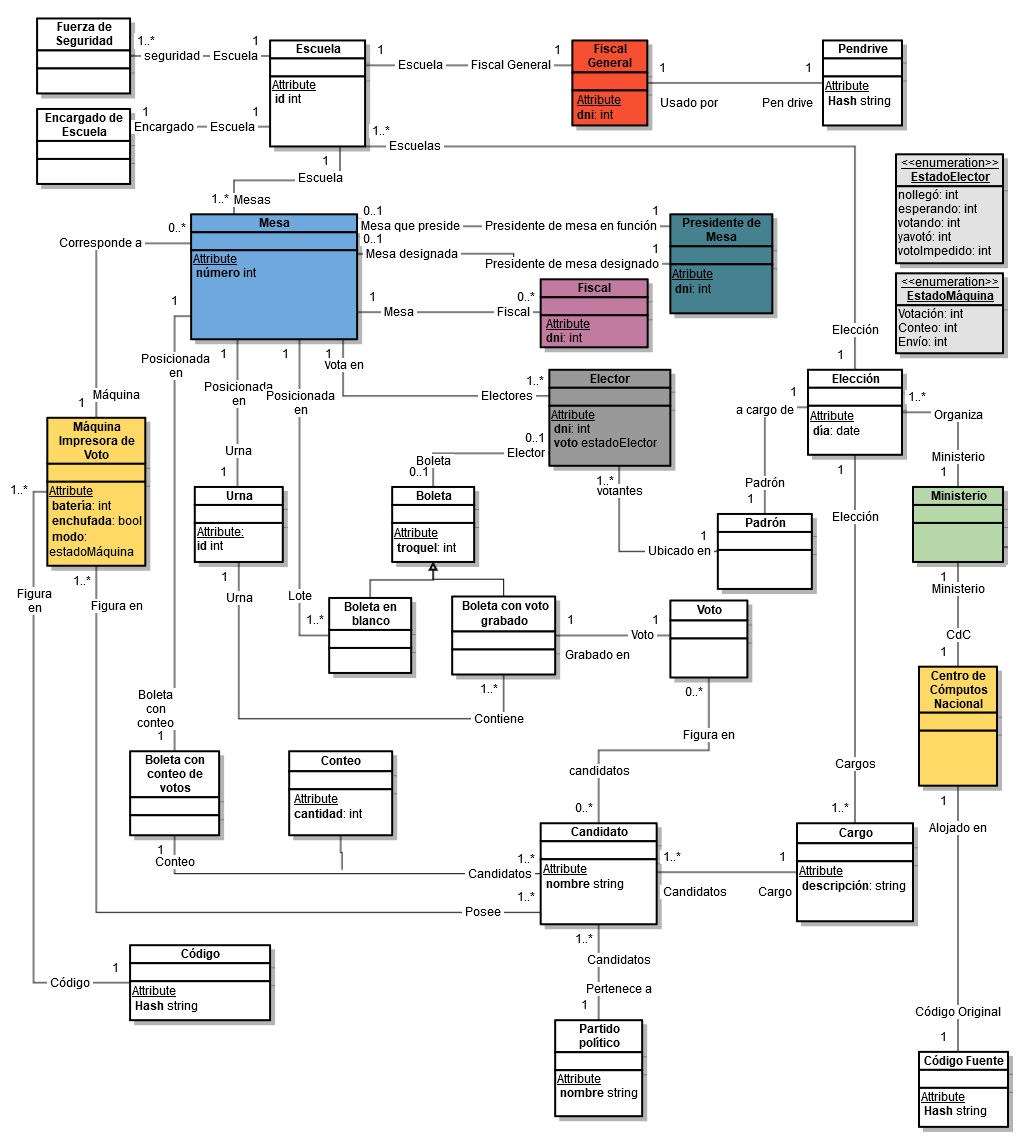
\includegraphics[scale=0.64]{imagenes/clases.png}
  \end{center}
\end{figure}

\newpage
\subsubsection{OCL}


\subsubsection*{Mesa}

\textit{context Mesa
inv}
\begin{enumerate}

\item Los n\'umeros de las mesas son únicos.

$Mesa.AllInstances \rightarrow forAll(m_1, m_2 | m_1<>m_2$ implies $m_1.numero <> m_2.numero))$

\item  No hay dos mesas con el mismo fiscal.\textcolor{red}{Preguntar si esto esta bien...}

$Mesa.AllInstances \rightarrow forAll(m_1, m_2 | m_1<>m_2$ implies $m_1.Fiscal.dni <> m_2.Fiscal.dni))$

\item No hay dos mesas con electores en común.

$Mesa.AllInstances \rightarrow \\
 forAll(m_1, m_2 | m_1<>m_2$ implies $m_1.Electores \rightarrow \\
 	forAll(e_1 | m_2.Electores \rightarrow Select(e_2 | e_2 <> e_1) \rightarrow Size() == 0))$

\item No hay dos mesas con el mismo presidente de mesa.

$Mesa.AllInstances \rightarrow \\
forAll(m_1, m_2 | m_1<>m_2$ implies $ \\ m_1.PresidenteDeMesaDesignado.dni <> m_2.PresidenteDeMesaDesignado.dni))$

\item Los presidentes de mesa votan en la misma mesa que son presidentes.

$self.Electores \rightarrow Select(e | self.PresidenteDeMesaDesignado.dni == e.dni) \rightarrow Size() ==1$


\item La cantidad de Boletas Sin voto grabado y con voto grabado de la mesa debe ser mayor o igual a la cantidad de electores de dicha mesa.

$self.Lote \rightarrow Size() + self.Urna.Contiene \rightarrow Size () \geq self.Electores \rightarrow Size()$

\item La cantidad de Boletas Con voto grabado de la mesa debe ser menor o igual a la cantidad de electores de dicha mesa.

$self.Urna.Contiene  \rightarrow  Size() \leq self.Electores \rightarrow Size()$

\item Si la máquina está en modo votación es porque s\'olo un elector, o ninguno, está votando.

$self.Maquina.modo == votacion$ implies $ \\
self.Electores \rightarrow select(e | e.voto == votando) \rightarrow Size() \leq 1$

\item Si la máquina está en modo conteo es porque no hay ningún elector de la mesa votando o esperando para votar.\textcolor{red}{Ver OR}

$self.Maquina.modo == votacion$ implies $ \\
self.Electores \rightarrow \\
select(e | e.voto == votando OR e.voto == esperando) \rightarrow Size() = 0$

\item La máquina de la mesa puede estar en modo votación o conteo pero no en envio.\textcolor{red}{Ver !}

$!self.Maquina.modo == envio$

\item No puede haber un fiscal y un presidente de mesa con el mismo dni.

$self.Fiscales \rightarrow \\
select(f | f.dni == self.PresidenteDeMesaEnFuncion.dni OR \\
f.dni == self.PresidenteDeMesaDesignado.dni) \rightarrow \\
Size() == 0 $


\end{enumerate}

\subsubsection*{Boleta}
\begin{enumerate}

\item Los id de las boletas son únicos.

$Boleta.AllInstances() \rightarrow select(b_1, b_2 | b_1 <> b_2 $ implies $ b_1.troquel <> b_2.troquel)$

\item La boleta con voto grabado tiene elector.


\item Si un elector tiene una boleta en blanco, entonces esta boleta está en la mesa que el elector vota.\textcolor{red}{Ver AND}

$self.IsKindOf(BoletaEnBlanco)? AND self.Elector \rightarrow Size() == 1 $ implies $\\
self.PosicionadaEn.numero == self.Elector.VotaEn.numero$

\item Si un elector tiene una boleta con voto grabado, entonces esta boleta está en la urna que el elector vot\'o.

$self.IsKindOf(BoletaConVotoGrabado)? $ implies $\\
self.Urna.PosicionadaEn.numero == self.Elector.VotaEn.numero$

\end{enumerate}


\subsubsection*{Conteo}

\begin{enumerate}

\item La boleta con conteo realmente tiene la información de las boletas de la urna (o sea la suma de los candidatos que hayan votado).
$self.Cantidad == \\
self.BoletaConConteodeVotos.mesa.boletaConVotoGrabado \rightarrow \\
select(b | b.voto.candidato  \rightarrow exist(c | c==self.candidato)) \rightarrow size() $
\end{enumerate}

\subsubsection*{Voto}
\begin{enumerate}
\item No tiene dos candidatos con el mismo cargo.

\item No tiene dos candidatos con el mismo nombre.
\end{enumerate}

\subsubsection*{Urna}
\begin{enumerate}
\item Las boletas con voto grabado de la urna son sólo de votantes de la mesa que figura la urna.
\item En una misma urna no hay dos boletas con el mismo elector.    
\item Los id de las urnas son únicos.
\end{enumerate}

\subsubsection*{Escuela}
\begin{enumerate}
\item Los id de las mesas son únicos.
\item No puede haber un fiscal general y un fiscal con el mismo dni.
\item No puede haber un fiscal general y un presidente de mesa con el mismo dni.
\end{enumerate}

\subsubsection*{M\'aquina Impresora de Voto}
\begin{enumerate}
\item Los candidatos de todas las máquinas son los mismos.

\end{enumerate}

\subsubsection*{Elector}
\begin{enumerate}
\item Los dni de los electores son únicos.
\item El elector puede no tener ninguna boleta, tener una vacía o tener una con voto.
\item No puede haber un elector y una persona que no figura en el padrón con el mismo dni.
\item Si el elector no llegó, está esperando o no lo dejaron votar no tiene boleta.
\item Si el elector está votando tiene una boleta en blanco.
\item Si el elector ya votó tiene una boleta con voto grabado.
\end{enumerate}

\subsubsection*{Partido Pol\'itico}
\begin{enumerate}
\item No hay dos partidos políticos con ningún candidato en común.
\end{enumerate}

\subsubsection*{Centro de C\'omputos}
\begin{enumerate}
\item Hay uno solo.
\end{enumerate}

\subsubsection*{C\'odigo}
\begin{enumerate}
\item El hash del código es el mismo del hash del código fuente.   
\item El hash del código es el mismo del hash de todos los pendrives de los fiscales.   
\end{enumerate}  

\subsubsection*{Ministerio}
\begin{enumerate}
\item Hay un solo ministerio.
\end{enumerate}

\subsubsection*{Equipo T\'ecnico}
\begin{enumerate}
\item Hay uno sólo.
\end{enumerate}

\subsubsection*{Presidente de Mesa}
\begin{enumerate}
\item Si el presidente de mesa del ministerio está presente, no hay presidente ad hoc.
\item Si la mesa tiene un solo presidente de mesa, tiene que ser el de Ministerio.
\item Si hay dos presidentes, el del ministerio debe estar ausente.
\item Si alguien voto, debe haber votado el presidente mesa antes (El Ad hoc si la mesa tiene dos presidentes, o el del ministerio si tiene uno solo).
\end{enumerate}

\subsubsection*{Candidato}
\begin{enumerate}
\item Los id de los candidatos son únicos.
\end{enumerate}


\newpage

\subsection{Preparación}

Ya presentados el diagrama de contexto y el de clases podemos pasar a analizar para cada una de las etapas presentadas en la introducción mediante los distintos diagramas ya presentados.

\subsubsection{Diagrama de actividad}


\begin{figure}[h!]
\centering
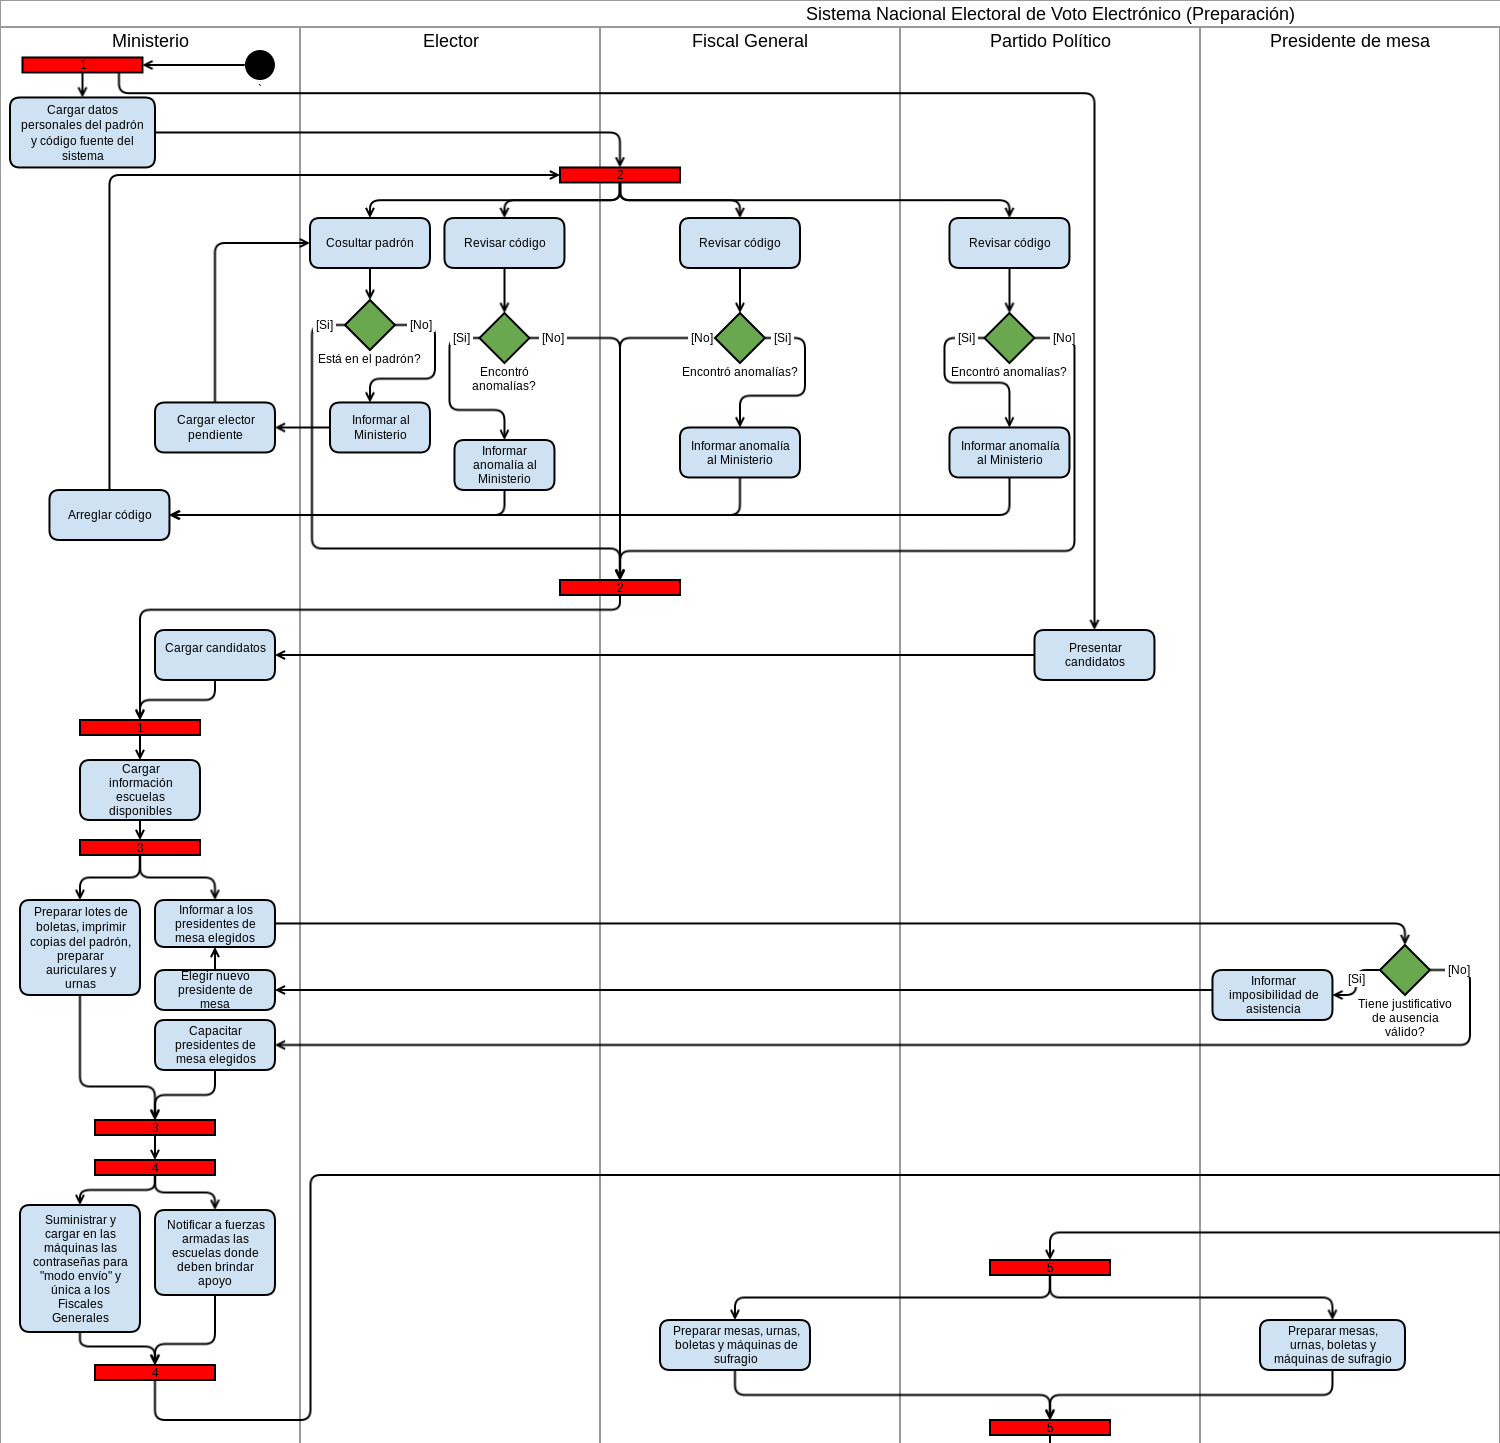
\includegraphics[scale=0.5]{imagenes/actividad/actividadPreparacion1}
%\captionof{figure}{Diagrama de actividad}
\end{figure}

\newpage

\begin{figure}[h!]
\centering
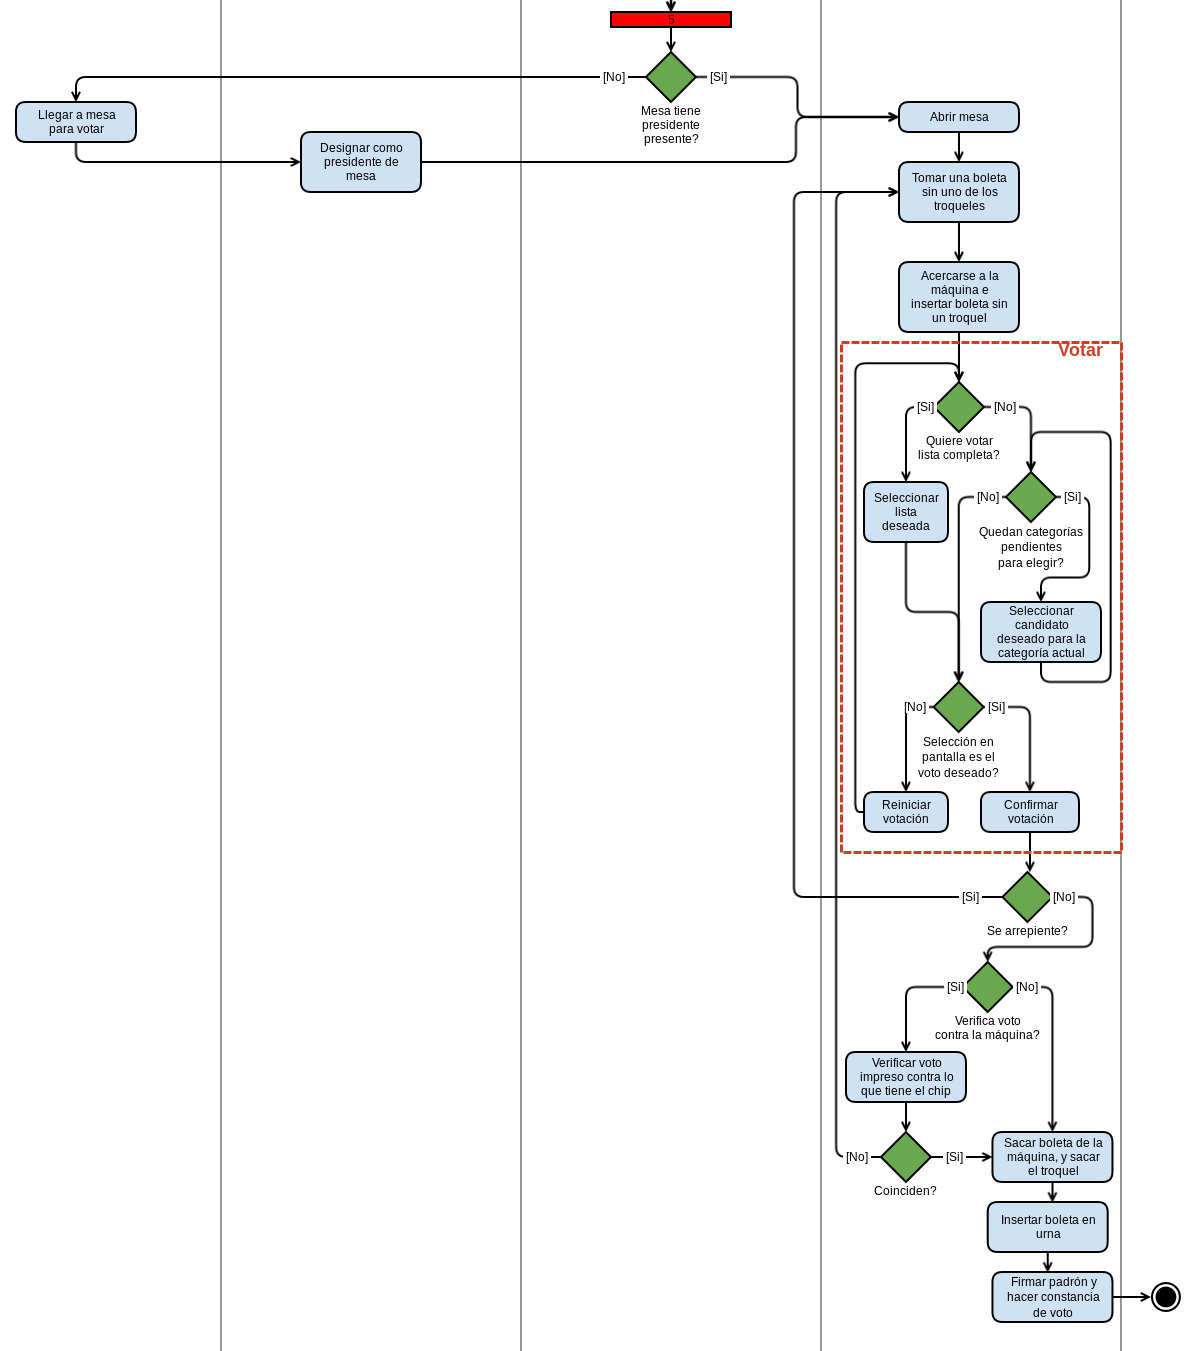
\includegraphics[scale=0.5]{imagenes/actividad/actividadPreparacion2}
\end{figure}

\begin{figure}[h!]
\centering
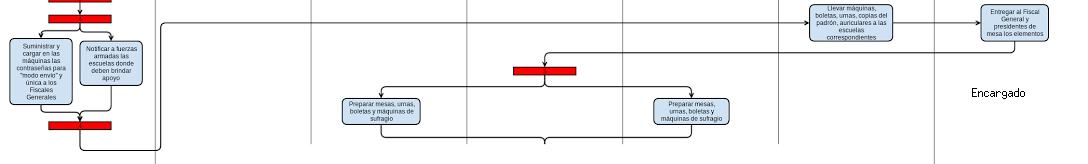
\includegraphics[scale=0.45]{imagenes/actividad/actividadPreparacion3}
\end{figure}

\newpage

Lo primero que se puede notar en el diagrama de actividad, es la división en 2 partes de esta sección. Por un lado, tenemos la verificación del código y la carga del padrón. Luego, pasamos a la carga de candidatos y asignaciòn de escuelas. Seguido de la asignaciòn de presidentes de mesa. Fionalmente se prepara todo para el día de la elección. Es importante notar como especificamos anteriormente que el voto del presidente de mesa es parte de esta instancia. 

Todas etapas tienen limites temporales definidos en relación a la elección, para modelarlos utilizaremos máquinas de estado finitas.

Finalmente en este diagramo definimos la acciòn de votar, si bien es algo de la etapa siguiente y hablaremos más de ella posteriormente, al definir el voto del presidente de mesa como el ultimo paso del proceso de preparaciòn fue necesario definirlo aquí.


\newpage
\subsubsection{Máquina de estado finito}

Para esta sección fue necesario construir 2 máquinas de estado.

%\begin{figure}[h!]
%\centering
%\includegraphics[scale=0.45]{}
%\captionof{figure}{Máquina de fechas limite}
%\end{figure}

Esta máquina de estado nos define los tiempos de la etapa, es decir enmarca los tiempos de los casos de uso presentados anteriormente. Es importante notar que las transiciones marcadas en esta FSM corresponden a las acciones mostradas en el diagrama de actividad con el mismo nombre.

%\begin{figure}[h!]
%\centering
%\includegraphics[scale=0.45]{}
%\captionof{figure}{Máquina de elección aleatoria de presidente de mesa}
%\end{figure}

A su vez, nos resultó interesante modelizar la selección aleatoria de presidentes de mesa utilizando FSM. Ya que deja bien en claro que solo se puede elegir uno.

\newpage
\subsubsection{Casos de uso}

Veamos primero el diagrama de casos de uso y luego veremos el detalle de los distintos casos de uso.


Es importante notar que el detalle de casos de uso, nos interioriza mucho en mucho de lo mencionado anteriormente en el diagrama de actividad. 


\begin{figure}[h!]
\centering
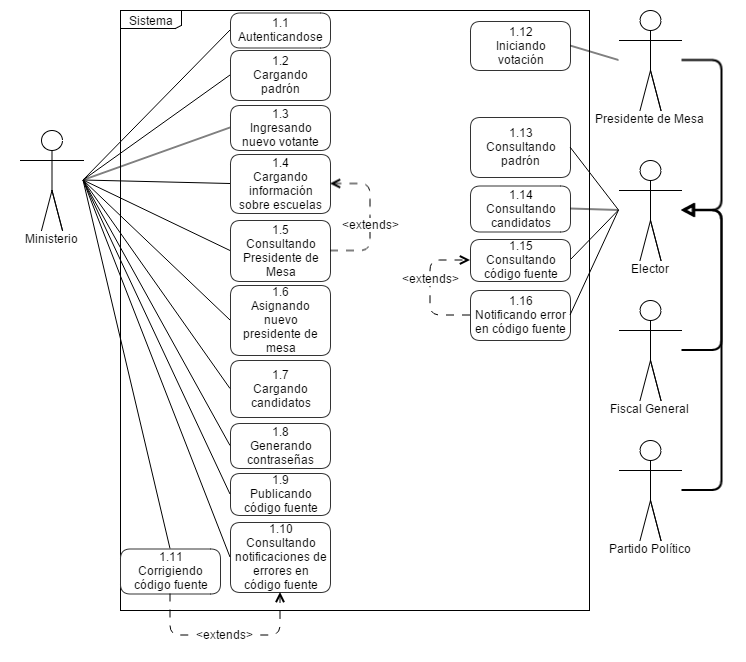
\includegraphics[scale=0.45]{imagenes/CU/casosdeusopreparacion}
%\captionof{figure}{Máquina de elección aleatoria de presidente de mesa}
\end{figure}



Al ver el diagrama, se nota algo interesante. Muchos agentes distintos terminan teniendo los mismos casos de uso que el elector. Si bien anteriormente tuvimos que distinguirlos y fue importante hacerlo, por sus interacciones esternas al sistema, cuando interactuan con el sistema son lo mismo que un elector.

Nos muestra también la importancia del diagrama de contexto para identificar agentes que quizas no interactuen con el sistema pero son escenciales a la construcción del mismo.

\newpage

\textbf{1.1 Caso de Uso: Autenticandose}

\textbf{Actores:} Ministerio

\textbf{Pre:} -

\textbf{Post:} El ministerio se encuentra autenticado en el sistema web.
\begin{table}[h!]
	
 \begin{tabular}{|p{7.5cm} | p{7.5cm}|} 
 \hline
 \textbf{Curso normal} & \textbf{Curso Alternativo} \\
 \hline
 %\hline
 1. El ministerio ingresa al sistema web. & \\
 \hline
 
 2. El sistema le pide usuario y contraseña para ingresar. & \\
 \hline 
 3. El ministerio ingresa usuario y contraseña, y elige la opción “Ingresar”. & \\
 \hline 
 4. La información se valida, y se muestra el menú principal. & 
4.1. La información de inicio no es correcta, por lo que se muestra un mensaje de error. Ir al paso 2.
\\
 \hline 
 5. Fin de CU. & \\

 \hline
 \end{tabular}

\end{table}


\textbf{1.2 Caso de uso: Cargando padrón}

\textbf{Actor}: Ministerio

\textbf{Pre}: El ministerio se encuentra autenticado en el sistema, el padrón no fue cargado, y todavía no pasó la fecha límite para modificaciones al padrón.

\textbf{Post}: El padrón se encuentra cargado en el sistema y puede ser consultado desde la web.

\begin{table}[h!]
	
 \begin{tabular}{|p{7.5cm} | p{7.5cm}|} 
 \hline
 \textbf{Curso normal} & \textbf{Curso Alternativo} \\
 \hline
1. El ministerio importa el padrón suministrando un archivo con todos los datos de los ciudadanos capacitados para votar.
El archivo importado es de formato .csv, con las siguientes columnas: Nombres, Apellidos, DNI, Dirección, Ciudad, Provincia y Sexo. & \\
\hline

2. El sistema guarda los datos y los publica en la web, para que sean consultados. &
2.1. Si ocurre un error durante la importación, mostrar mensaje de error e ir al fin del caso de uso. \\
\hline
3. Fin de CU. & \\
\hline
 \end{tabular}

\end{table}


\textbf{1.3 Caso de Uso: Ingresando nuevo votante}

\textbf{Actores:} Ministerio

\textbf{Pre:} El ministerio se encuentra autenticado en el sistema, el padrón se encuentra cargado en el sistema, y puede ser consultado desde la web.

\textbf{Post:} El padrón se actualiza en el sistema, agregando al nuevo votante.
\begin{table}[h!]
	
 \begin{tabular}{|p{7.5cm} | p{7.5cm}|} 
 \hline
 \textbf{Curso normal} & \textbf{Curso Alternativo} \\
 \hline

1. El ministerio ingresa los datos del nuevo votante en un formulario. & \\
\hline

2. El ministerio elige la opción de “Cargar votantes”. & \\
\hline

3. Se actualizan los datos en el sistema. & 3.1. Si existe un error en la carga, se muestra un mensaje con el error. Ir al paso 2. \\
\hline
4. Fin de CU. & \\
 \hline
 \end{tabular}

\end{table}

\newpage

\textbf{1.4 Caso de uso: Cargando información sobre escuelas}

\textbf{Actor:} Ministerio

\textbf{Pre:} El ministerio se encuentra autenticado en el sistema, y pasó la fecha establecida para la modificación del padrón.

\textbf{Post:} El sistema posee la información de los electores y sus mesas correspondientes, y además designó un presidente de mesa para cada una. Esta información se encuentra consultable en la web.


\begin{table}[h!]
	
 \begin{tabular}{|p{7.5cm} | p{7.5cm}|} 
 \hline
 \textbf{Curso normal} & \textbf{Curso Alternativo} \\
 \hline

1. El ministerio importa la información sobre las escuelas suministrando un archivo con todos los datos de las escuelas. El archivo importado es de formato .csv, con las siguientes columnas: Nombre, Dirección, Ciudad, Provincia y Cantidad de aulas. & \\
\hline

2. El sistema guarda los datos importados y asigna a los electores a las escuelas más cercanas, asignando una mesa a cada uno. &
2.1. Si ocurre un error durante la importación, mostrar mensaje de error e ir al fin del caso de uso. \\
\hline
3. El sistema aleatoriamente elige un presidente de mesa, priorizando a aquellos que no lo fueron previamente. & \\
\hline

4. El sistema ofrece la posibilidad de consultar los presidentes de mesa seleccionados. &
4.1. En caso de ocurrir un error, mostrar mensaje de error e ir a fin del caso de uso. \\
\hline
5. Si se elige la opción, se extiende con el CU\textbf{1.5 Consultando presidentes de mesa}. & \\
\hline

6. El sistema publica la información en la web para que pueda ser consultada. & \\
\hline

7. Fin de CU. & \\
\hline

 \end{tabular}

\end{table}


\textbf{1.5 Caso de Uso: Consultando presidentes de mesa}

\textbf{Actores:} Ministerio 

\textbf{Pre:} El ministerio se encuentra autenticado en el sistema, las mesas y los presidentes de mesa se encuentra publicados.

\textbf{Post:} El ministerio conoce a los presidentes de mesa.
\begin{table}[h!]
	
 \begin{tabular}{|p{7.5cm} | p{7.5cm}|} 
 \hline
 \textbf{Curso normal} & \textbf{Curso Alternativo} \\
 \hline

1. El ministerio selecciona la pestaña de consulta de presidentes de mesa. & \\
\hline
2. El ministerio consulta en el sistema los presidentes asignados a cada mesa. & \\
\hline
3. Fin de CU. & \\
\hline
 \end{tabular}

\end{table}

\textbf{1.6 Caso de Uso: Asignando nuevo presidente de mesa}

\textbf{Actores:} Ministerio 

\textbf{Pre:} El ministerio se encuentra autenticado en el sistema, las mesas y los presidentes de mesa se encuentran publicados, y un presidente de mesa envió una notificación explicando que no puede estar presente. La notificación se envió llamando a la línea gratuita del ministerio.

\textbf{Post:} Se asigna un nuevo presidente a una mesa.

\newpage

\begin{table}[h!]
	
 \begin{tabular}{|p{7.5cm} | p{7.5cm}|} 
 \hline
 \textbf{Curso normal} & \textbf{Curso Alternativo} \\
 \hline

1. El ministerio activa la opción de una nueva asignación de presidente de mesa para la mesa afectada. & \\
\hline

2.  El sistema aleatoriamente elige un presidente de mesa, descartando al presidente ya elegido, y priorizando a aquellos que no lo fueron previamente. & \\
\hline


3. Fin de CU. & \\
\hline



 \end{tabular}

\end{table}

\textbf{Caso de uso: 1.7 - Cargando candidatos}

\textbf{Actor:} Ministerio

\textbf{Pre:} El ministerio se encuentra autenticado en el sistema, y ya pasó la fecha de presentación de candidatos.

\textbf{Post:} Los candidatos se encuentran cargados en el sistema y son consultables vía web. Además, las máquinas de sufragio tienen cargados los candidatos.
\begin{table}[h!]
	
 \begin{tabular}{|p{7.5cm} | p{7.5cm}|} 
 \hline
 \textbf{Curso normal} & \textbf{Curso Alternativo} \\
 \hline
1. El ministerio importa los candidatos suministrando un archivo con todos los datos cada uno y su respectivo candidato. & \\
\hline

2. El sistema guarda los datos y los publica en la web, para que sean consultados. &
2.1. Si ocurre un error durante la importación, mostrar mensaje de error e ir al fin del caso de uso. \\
\hline
3. Luego, el ministerio carga en todas las máquinas de sufragio los candidatos para el día de la elección. & \\
\hline

4. Fin de CU. & \\
\hline
\end{tabular}
\end{table}

\textbf{Caso de uso: 1.8 - Generando contraseñas}

\textbf{Actor:} Ministerio

\textbf{Pre:} El ministerio se encuentra autenticado en el sistema, y las escuelas se encuentran cargadas.

\textbf{Post:} El ministerio ahora posee una contraseña general para entrar a modo envío y una contraseña para cada fiscal. Además, las máquinas de sufragio tienen cargadas la contraseña para entrar a Modo Envío.

\begin{table}[h!]
	
 \begin{tabular}{|p{7.5cm} | p{7.5cm}|} 
 \hline
 \textbf{Curso normal} & \textbf{Curso Alternativo} \\
 \hline

1. El ministerio selecciona la opción de Generar Contraseñas. & \\
\hline

2. El sistema genera una contraseña general para que todas las computadoras de sufragio puedan entrar en Modo Envío y una contraseña diferente para cada fiscal. & \\
\hline

3. Luego, el ministerio carga en todas las máquinas de sufragio la contraseña para entrar en Modo Envío. & \\
\hline

4. Fin de CU. & \\
\hline

\end{tabular}
\end{table}
\textbf{Caso de uso: 1.9 - Publicando código fuente}

\textbf{Actor:} Ministerio

\textbf{Pre:} El ministerio se encuentra autenticado en el sistema y todavía no es el día de las elecciones.

\textbf{Post:} El código fuente se encuentra cargado en la web para ser consultado. 

\newpage

\begin{table}[h!]
	
 \begin{tabular}{|p{7.5cm} | p{7.5cm}|} 
 \hline
 \textbf{Curso normal} & \textbf{Curso Alternativo} \\
 \hline
 
1. Selecciona la opción de publicar código fuente. & \\
\hline

2. El ministerio carga el código fuente. & \\
\hline

3. El ministerio publica el código fuente. & \\
\hline

4. Fin de CU. & \\
\hline
\end{tabular}
\end{table}

\textbf{1.10 Caso de Uso: Consultando notificaciones de error en código fuente}

\textbf{Actores:} Ministerio 

\textbf{Pre:} El ministerio se encuentra autenticado en el sistema y el código fuente se encuentra publicado.
\textbf{Post:} El ministerio conoce las notificaciones de error sobre el código fuente.

\begin{table}[h!]
	
 \begin{tabular}{|p{7.5cm} | p{7.5cm}|} 
 \hline
 \textbf{Curso normal} & \textbf{Curso Alternativo} \\
 \hline


1. El ministerio selecciona la pestaña de notificaciones. & \\
\hline


2. El ministerio ministerio revisa todas las notificaciones cargadas en el sistema. & \\
\hline


3. Si se decide corregir uno de los errores cargados, se extiende con el CU \textbf{1.11 Corrigiendo código fuente}. & \\
\hline


4. Fin de CU. & \\
\hline




 \end{tabular}

\end{table}


\textbf{Caso de uso: 1.11 - Corrigiendo código fuente}

\textbf{Actor:} Ministerio

\textbf{Pre:} El ministerio se encuentra autenticado en el sistema, el código fuente se encuentra publicado, el ministerio recibió un aviso de un error en el código fuente y se encontró una solución.
\textbf{Post:} El código fuente se actualiza en el sistema, corrigiendo los errores que existían.

\begin{table}[h!]
	
 \begin{tabular}{|p{7.5cm} | p{7.5cm}|} 
 \hline
 \textbf{Curso normal} & \textbf{Curso Alternativo} \\
 \hline



1. El ministerio elige la pestaña de modificación del código fuente. & \\
\hline

2. El ministerio actualiza el código fuente en el sistema web y publica la actualización. & \\
\hline

3. El ministerio actualiza el código fuente en todas las máquinas de sufragio. & \\
\hline


4. El ministerio marca en el sistema que la notificación del error solucionado fue resuelta. & \\
\hline

5. Fin de CU. & \\
\hline

\end{tabular}
\end{table}

\textbf{1.12 Caso de Uso: Iniciando votación}

\textbf{Actores:} Presidente de mesa

\textbf{Pre:} Es el día de la votación y ya se encuentra todo preparado en la mesa.

\textbf{Post:} La máquina ya se puede utilizar para votar, y el presidente de mesa ya votó.

\begin{table}[h!]
	
 \begin{tabular}{|p{7.5cm} | p{7.5cm}|} 
 \hline
 \textbf{Curso normal} & \textbf{Curso Alternativo} \\
 \hline

1. El presidente de mesa conecta la máquina de sufragio a la red eléctrica. & \\
\hline
2. El presidente de mesa prende la máquina de sufragio y activa el modo votación. & \\
\hline
3. El presidente de mesa vota de acuerdo a lo explicado en el CU \textbf{2.12 Votando} del Elector. & \\
\hline
4. Fin de CU.& \\
\hline



 \end{tabular}

\end{table}

\newpage

\textbf{1.13Caso de Uso:  Consultando padrón}

\textbf{Actores:} Elector 

\textbf{Pre:} El padrón se encuentra publicado en la web. 

\textbf{Post:}  El elector conoce si se encuentra en el padrón.


\begin{table}[h!]
	
 \begin{tabular}{|p{7.5cm} | p{7.5cm}|} 
 \hline
 \textbf{Curso normal} & \textbf{Curso Alternativo} \\
 \hline

1. El elector ingresa al sistema web público del sistema. & \\
 \hline



2. Se busca en el padrón por su DNI. & \\
 \hline



3. Si se encuentra, ir a 5. & \\
 \hline



4. Si el elector no se encuentra en el padrón, se lo comunica al ministerio, y se extiende con CU Ingresando nuevo votante. & \\
 \hline



5. Fin de CU. & \\
 \hline


 \end{tabular}

\end{table}


	

\textbf{1.14 Caso de Uso: Consultando candidatos}

\textbf{Actores:} Elector 

\textbf{Pre:} Los candidatos fueron publicados.

\textbf{Post:}  El elector conoce los candidatos.
\begin{table}[h!]
	
 \begin{tabular}{|p{7.5cm} | p{7.5cm}|} 
 \hline
 \textbf{Curso normal} & \textbf{Curso Alternativo} \\
 \hline
 
1. El elector ingresa al sistema web público del sistema. & \\
 \hline



2. El elector visita la sección de candidatos de la web. & \\
 \hline


3. Fin de CU. & \\
 \hline


 \end{tabular}

\end{table}


\textbf{1.15 Caso de Uso: Consultando código fuente}

\textbf{Actores:} Elector

\textbf{Pre:} El código fuente se encuentra publicado en la web.

\textbf{Post:} El elector ahora conoce el código fuente.

\begin{table}[h!]
	
 \begin{tabular}{|p{7.5cm} | p{7.5cm}|} 
 \hline
 \textbf{Curso normal} & \textbf{Curso Alternativo} \\
 \hline
1. El elector ingresa al sistema web público del sistema. & \\
 \hline


2. El elector navega a la sección del código fuente. & \\
 \hline


3. El elector revisa el código fuente, en busca de posibles errores. & \\
 \hline


4. Si no encuentra errores, ir a 6. & \\
 \hline


5. Si encuentra un error, se extiende con el CU \textbf{1.16 Notificando error en el código fuente}. & \\
 \hline


6. Fin de CU. & \\
 \hline

 \end{tabular}

\end{table}

\newpage

\textbf{1.16 Caso de Uso: Notificando error en código fuente}

\textbf{Actores:}  Elector

\textbf{Pre:} El código fuente se encuentra publicado en la web, el elector se encuentra en el sistema web y ya consultó el código previamente.

\textbf{Post:} En el sistema ahora existe una nueva denuncia del código fuente.


\begin{table}[h!]
	
 \begin{tabular}{|p{7.5cm} | p{7.5cm}|} 
 \hline
 \textbf{Curso normal} & \textbf{Curso Alternativo} \\
 \hline
1. El elector navega a la sección de denuncias del código fuente. & \\
\hline


2. El elector llena un formulario, explicando las causas de la denuncia. Luego, elige la opción de “Enviar denuncia”. & \\
\hline


3. Se valida la información, y se carga en el sistema. & 3.1. Si existe un error en la carga del formulario, se muestra un mensaje de error. Ir al fin del caso de uso. \\
\hline
4. Fin de CU.& \\
\hline
 \end{tabular}

\end{table}


\newpage

\subsection{Sufragio}

La sección de sufragio, es una etapa donde se repite muchas veces un caso de uso. El de \textbf{Votar}, ya que todos los electores hacen lo mismo. Para modelizar este momento son necesarias distintas cotas temporales y una manera de componer esta acción muchas veces.

\subsubsection{Diagrama de actividad}

\begin{figure}[h!]
\centering
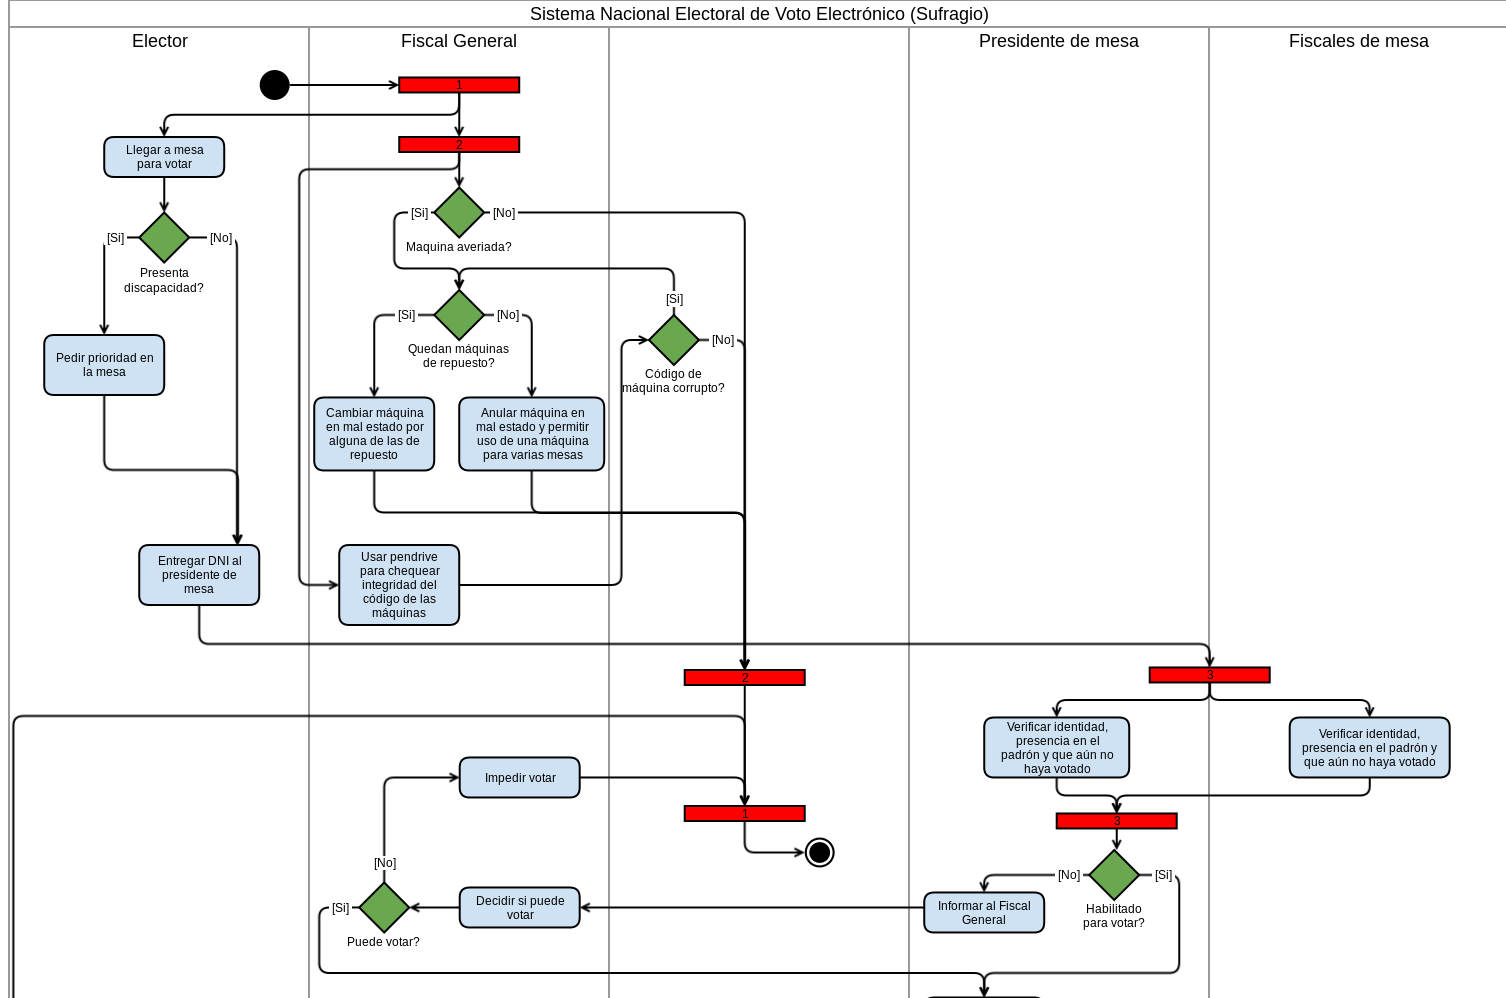
\includegraphics[scale=0.5]{imagenes/actividad/actividadSufragio1}
%\captionof{figure}{Diagrama de actividad}
\end{figure}

\begin{figure}[h!]
\centering
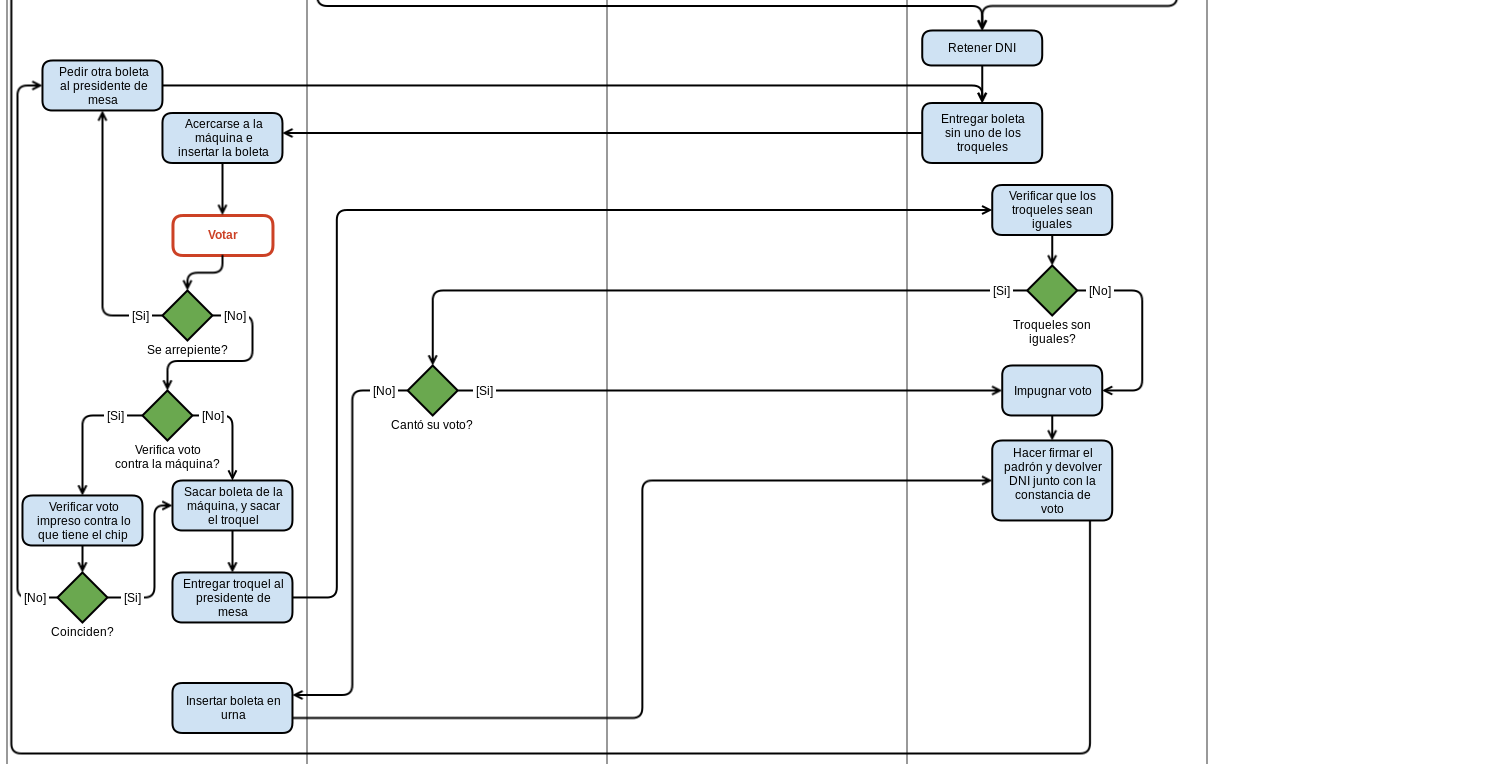
\includegraphics[scale=0.5]{imagenes/actividad/actividadSufragio2}
\end{figure}

\newpage

El diagrama de actividad nos da una primera visión del proceso de votación, vemos la interrelación entre los distintos agentes de una mesa y el elector. A su vez, comenzamos a ver la importancia de nuestro sistema en todo este esquema. Sin embargo, el diagrama de actividad no logra modelar bien la idea de una cola para votar con prioridad para discapacitados. Ni la posibilidad de muchos votantes. Por eso decidimos usar máquinas de estado finitas para modelar estos importantisimos conceptos a la hora de modelizar la votación.


\newpage
\subsubsection{Máquina de estado finito}

La idea aquí fue utilizar dos FSM, para modelizar que solo puede votar una persona a la vez y los horarios.

%\begin{figure}[H]
%\centering
%\includegraphics[scale=0.45]{}
%\captionof{figure}{Máquina de elección aleatoria de presidente de mesa}
%\end{figure}

La idea de esta máquina fue modelizar los siguientes conceptos:
\begin{itemize}
\item Solo un votante puede ocupar la máquina de sufragio correspondiente a su mesa al mismo tiempo (no hay dos usando la máquina en simultáneo).
\item El presidente de dicha mesa no puede atender a dos votantes en simultáneo.
\item Los votantes son llamados según el orden de llegada.
\item Los votantes discapacitados tienen prioridad.

\end{itemize}

Es importante notar que esto vale para los agentes de una mesa determinada en una escuela. Es decir que la composición de estas máquinas será de n electores por cada mesa de cada escuela.

%\begin{figure}[H]
%\centering
%\includegraphics[scale=0.45]{}
%\captionof{figure}{Máquina de elección aleatoria de presidente de mesa}
%\end{figure}

Esta FSM modela:
\begin{itemize}
\item El horario durante el que transcurre el sufragio es entre las 8 y las 18 hs.
\item El presidente de mesa/Fiscal General/fiscal deben esperar a que abran y cierren la escuela.
\item El presidente de mesa vota primero

\end{itemize}

\newpage

\subsubsection{Casos de uso}

\begin{figure}[h!]
  \begin{center}
    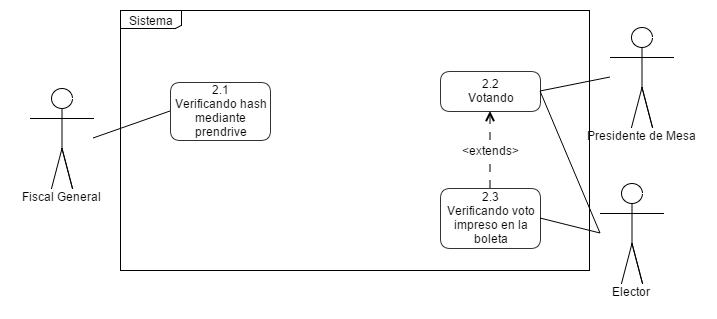
\includegraphics[scale=0.45]{imagenes/CU/casosdeusosufragio.png}
  \end{center}
\end{figure}

Vemos que los casos de uso para esta etapa son pocos, no hay una interacción muy grande con el sistema a nivel de 1 agente. Pero es importante notar que como vimos anteriormente son casos de uso que haran TODOS los electores, por lo tanto se usaran en grandes cantidades el caso de uso \textbf{votando}, que como vimos es una instancia compleja.

Entonces, en esta sección fue necesaria una interrelación de 3 diagramas para lograr modelar la acción de votar en una mesa. Y ahroa pasaremos a los detalles de caso de uso apra comprender aún más sobre este proceso.

\newpage

\textbf{Caso de uso: 2.1 - Verificando hash mediante pendrive}

\textbf{Actor:} Fiscal General
\textbf{Pre:} Es el día de las elecciones y el fiscal general posee el pendrive verificador.

\textbf{Post:} El hash se verifica y es correcto.

\begin{table}[h!]
	
 \begin{tabular}{|p{7.5cm} | p{7.5cm}|} 
 \hline
 \textbf{Curso normal} & \textbf{Curso Alternativo} \\
 \hline
	

1. El fiscal general se acerca a una máquina de sufragio e inserta el pendrive verificador en la misma. & \\
 \hline
2. Se ejecuta automáticamente el software dentro del pendrive, que busca el ejecutable en ejecución.& \\


3. El software del pendrive calcula el hash del ejecutable encontrado y lo compara con el hash esperado. & \\
\hline

4. Si coincide el hash, se quita el pendrive y el fiscal deja la máquina para que se siga votando normalmente. &
4.1. Si hash calculado no coindice con el esperado, se muestra en pantalla un mensaje de error. Ir a fin del caso de uso. \\
\hline
5. Fin de CU. & \\
\hline
\end{tabular}
\end{table}

\textbf{Caso de uso: 2.2 - Votando}

\textbf{Actor:} Elector, Presidente de Mesa

\textbf{Pre:} Es el día de las elecciones y la máquina de sufragio ya fue iniciada en modo votación.

\textbf{Post:} El elector imprimió su voto en una boleta.

\newpage

\begin{table}[h!]
	
 \begin{tabular}{|p{7.5cm} | p{7.5cm}|} 
 \hline
 \textbf{Curso normal} & \textbf{Curso Alternativo} \\
 \hline
1. Si el elector no necesita de asistencia por sonido para votar, ir al 6. & \\
\hline

2. El presidente de mesa acerca al elector a la máquina, inserta una boleta vacía en la máquina e inserta los auriculares en la máquina, la cual detecta los mismos y empieza a dictar los candidatos al elector. & \\
\hline

3. Por cada categoría, el elector escucha todos los candidatos, más la opción de votar en blanco. Cuando escucha la opción que desea elegir, toca cualquier lugar en la pantalla. & \\
\hline

4. Una vez finalizadas todas las categorías, se le dicta la elección al elector. Se le pregunta también si desea imprimir su voto. & \\
\hline

5. Si decide por “No”, ir a 3. Si decide por sí, ir al paso 7. & \\
\hline

6. Si el elector no necesita de asistencia, vota de acuerdo a lo mostrado en la sección “Votar” del Diagrama de Actividad. & \\
\hline

7. Una vez finalizada la elección, se imprime el voto en la boleta. Se carga la información en el chip, y se imprime en tinta una tabla donde se especifica qué candidato se votó para cada categoría. & \\
\hline

8. La máquina le recomienda al lector verificar su voto utilizando el lector. Si decide hacerlo, se extiende con el CU 2.3 - Verificando voto impreso en la boleta. & \\
\hline

9. Fin de CU. & \\
\hline

\end{tabular}
\end{table}
\textbf{Caso de uso: 2.3 - Verificando voto impreso en la boleta}

\textbf{Actor:} Elector

\textbf{Pre:} Es el día de las elecciones y acaba de votar.

\textbf{Post:} El elector confirma que su boleta indica que votó lo que le eligió.

\begin{table}[h!]
	
 \begin{tabular}{|p{7.5cm} | p{7.5cm}|} 
 \hline
 \textbf{Curso normal} & \textbf{Curso Alternativo} \\
 \hline
 1. El elector primero verifica que la boleta tenga imprenta en tinta la información correcta. & \\
\hline

2. Si es así, acerca la boleta al lector de la máquina de sufragio, apoyando la parte con el chip. De esta forma, verifica que lo mostrado en pantalla sea su elección. & \\
\hline

3. Si es así, el elector dobla la boleta asegurándose que la parte impresa en tinta no quede visible. & \\
\hline

4. Fin de CU. & \\
\hline
\end{tabular}
\end{table}

\newpage

\subsection{Conteo}

Llegamos, a la ultima sección. Ya terminada la elección es necesario ver comom contar los votos. Aquí el sistema toma un rol muy importante. A su vez tenemos algunos actores importantescomo el presidente de mesa y los fiscales que se entremezclan con el conteo automático.

\subsubsection{Diagrama de actividad}

\begin{figure}[h!]
\centering
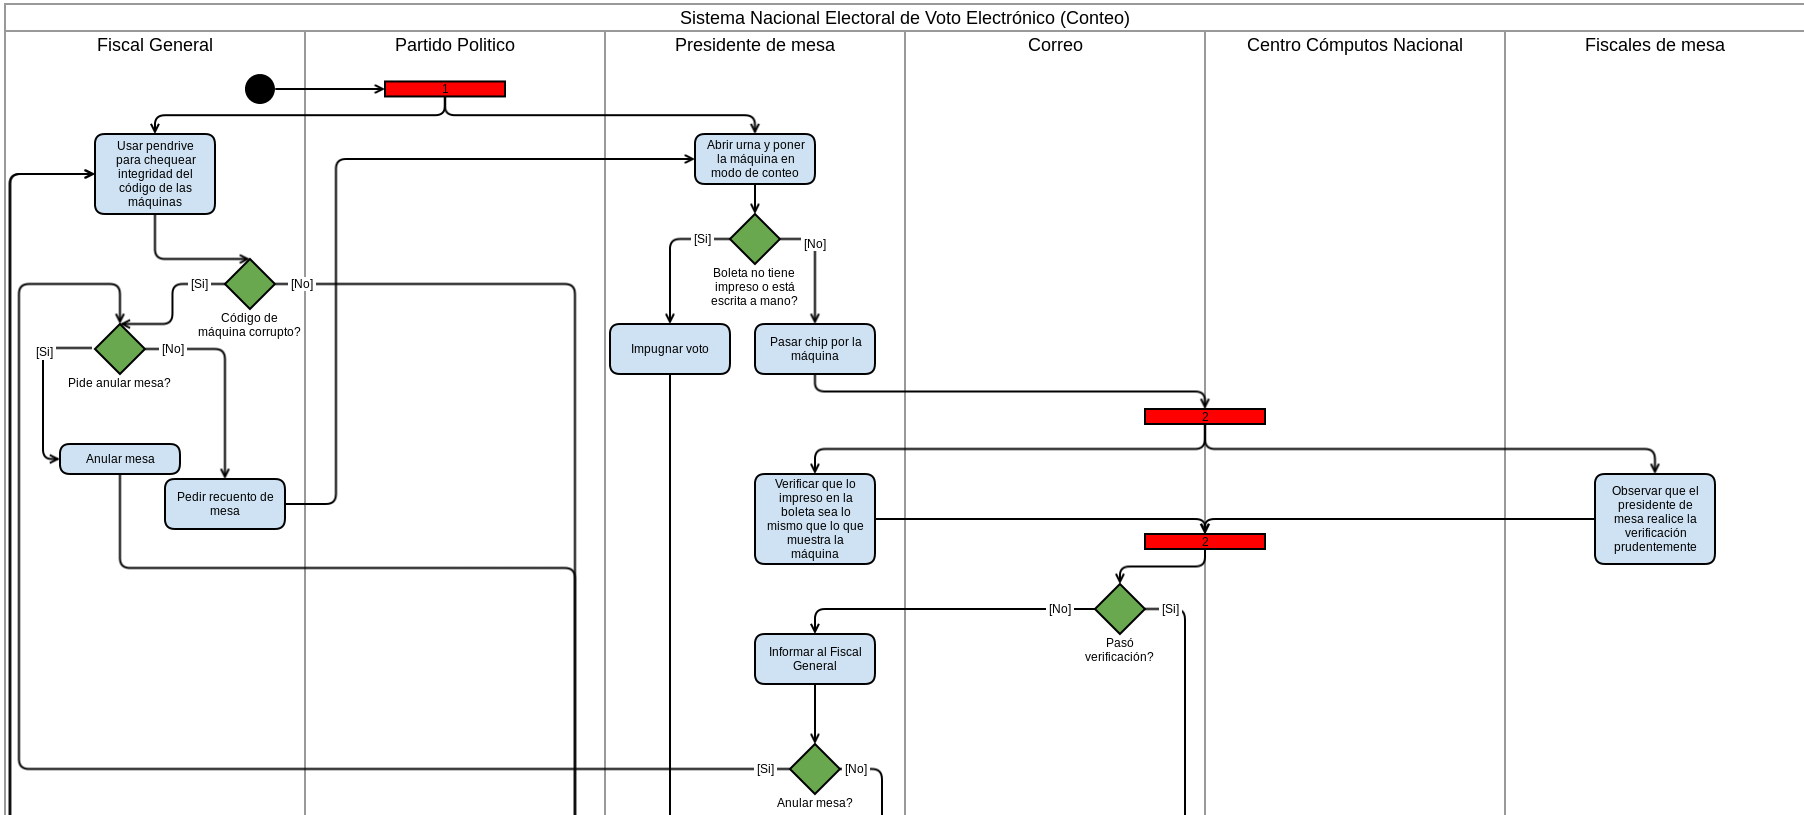
\includegraphics[scale=0.45]{imagenes/actividad/actividadConteo1}
%\captionof{figure}{Diagrama de actividad}
\end{figure}			


\begin{figure}[h!]
\centering
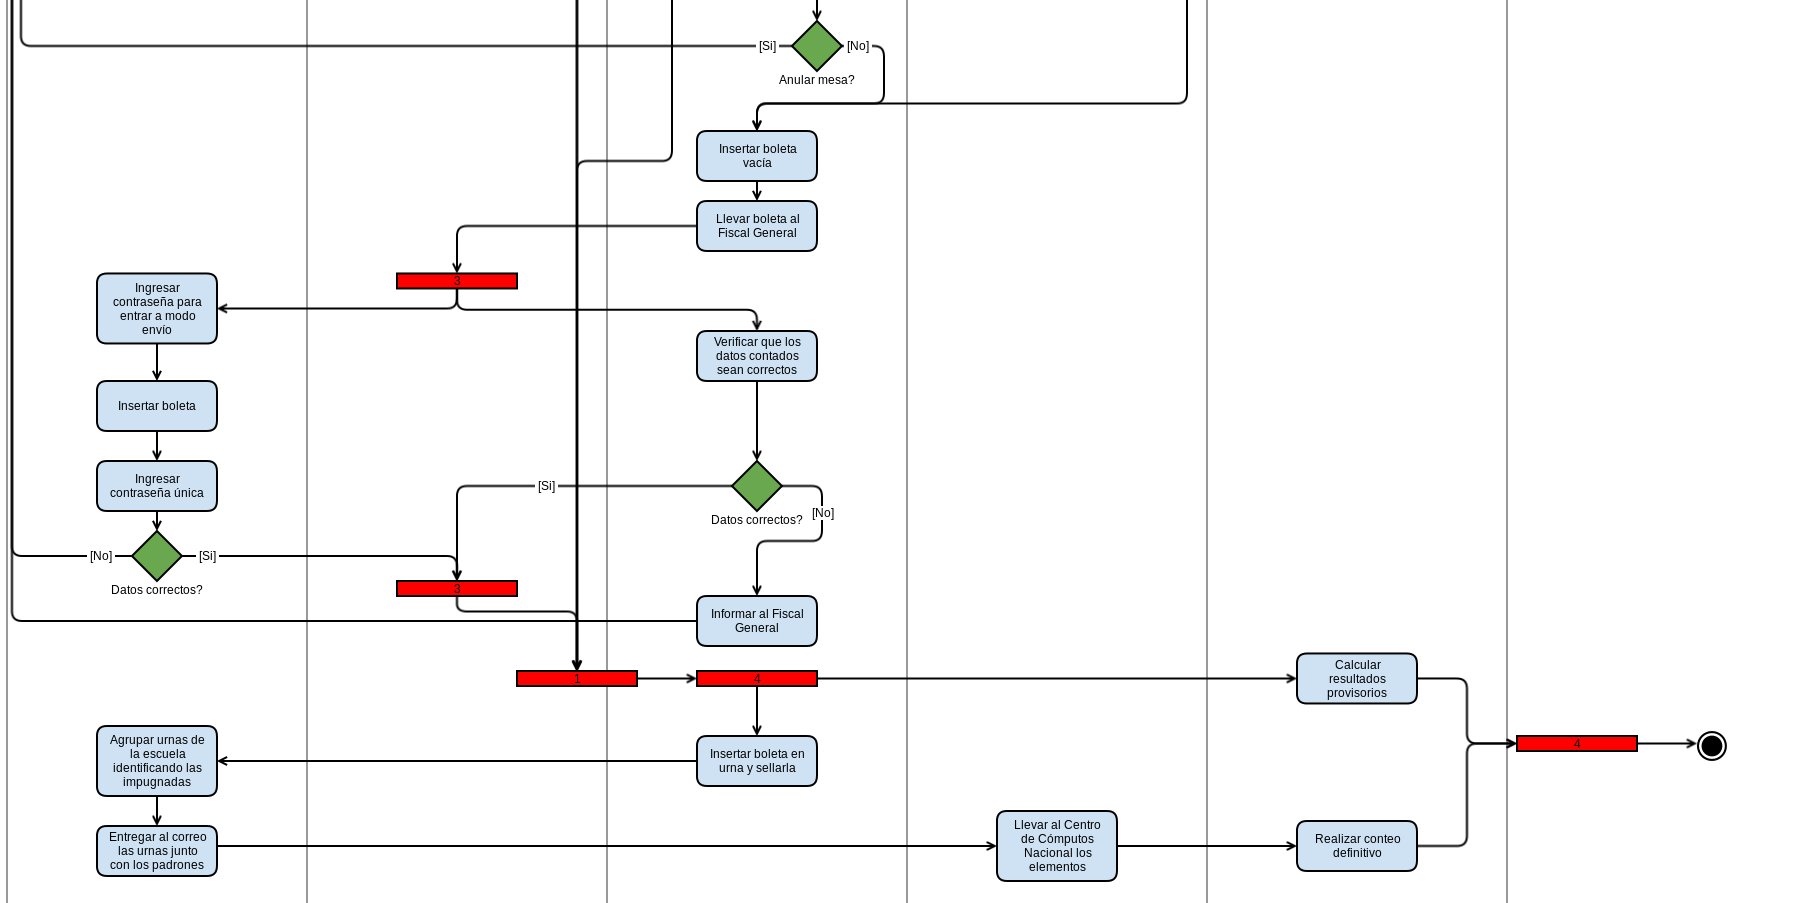
\includegraphics[scale=0.45]{imagenes/actividad/actividadConteo2}
\end{figure}

Aquí vemos como hay dos grandes acciones en esta etapa, por un lado poder auditar la máquina para ver qu\'e est\'a sucediendo, por otro lado el conteo. Una vez más el diagrama de actividad nos permite dar una forma de lo hechos pero no nos permite definar del todo como funciona el conteo ni la auditoria del mismo, para esto usaremos FSM de manera a darla más forma.

\newpage

\subsubsection{Máquina de estado finito}

%\begin{figure}[h!]
%\centering
%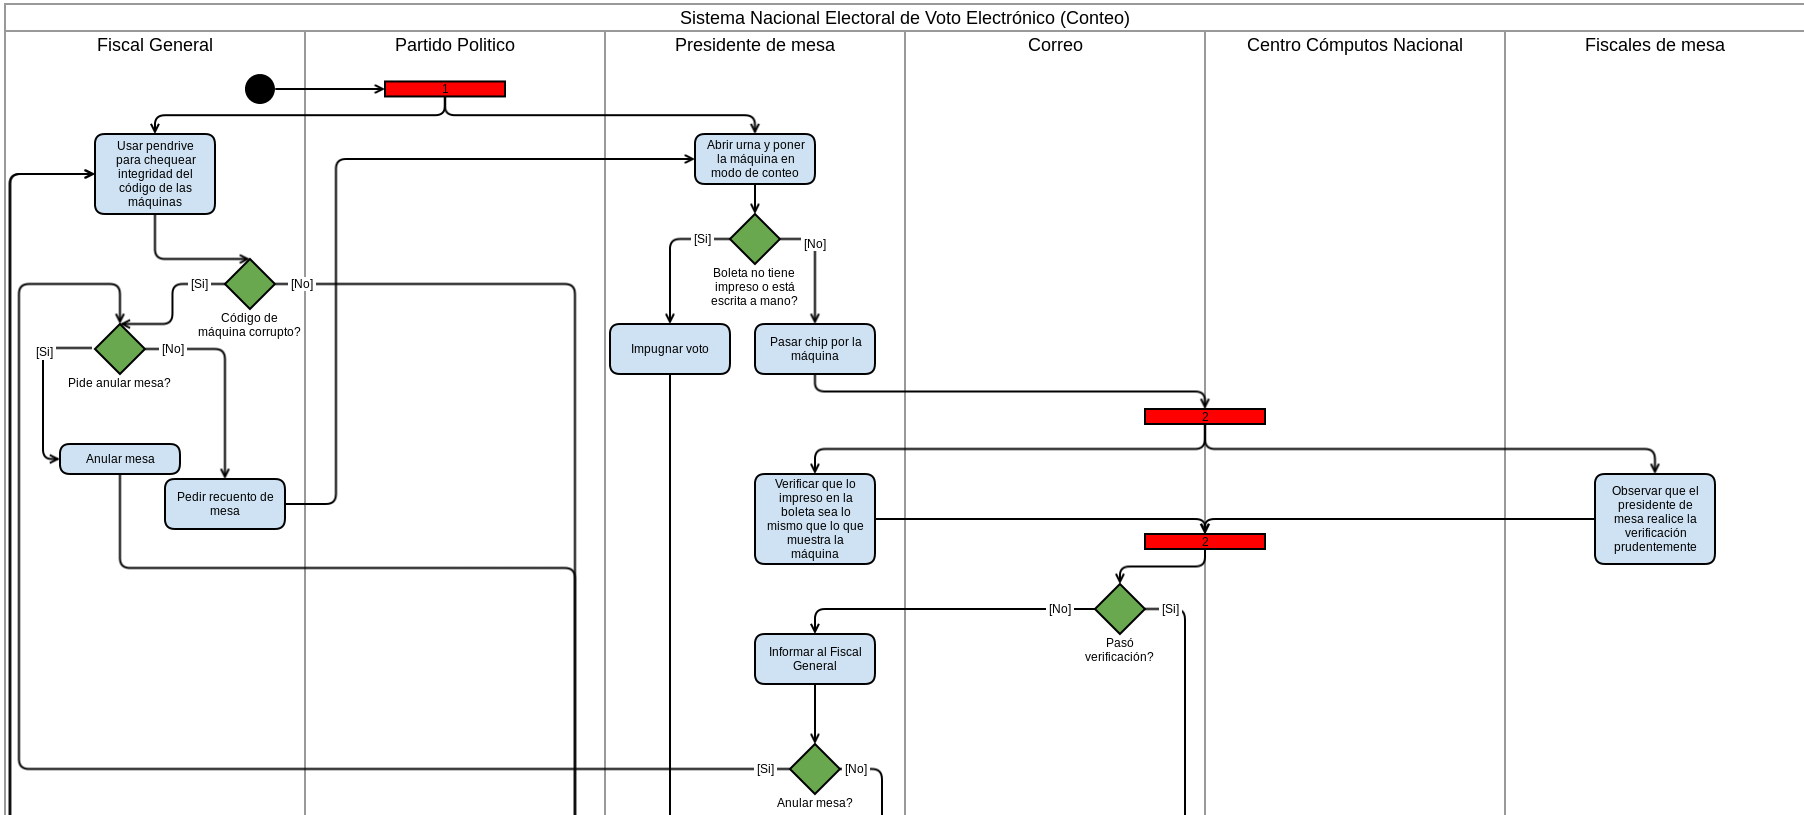
\includegraphics[scale=0.5]{imagenes/actividad/actividadConteo1}
%\captionof{figure}{Diagrama de actividad}
%\end{figure}			

Este modelo representa el proceso de conteo de una mesa. PAra modelizarlo realmente, es necesario hacer la composición de estos tres modelos. Es importante notar que Finaliza conteo representa todo la etapa de impresión y entrega de los datos mediante modo envio, ya que esto es una acción unica que se ve mucho mejor tanto en casos de uso como el diagrama de actividad no fue tomada en cuenta para este modelo y se comprimio en esa unica etiqueta.


\newpage

\subsubsection{Casos de uso}

\begin{figure}[h!]
\centering
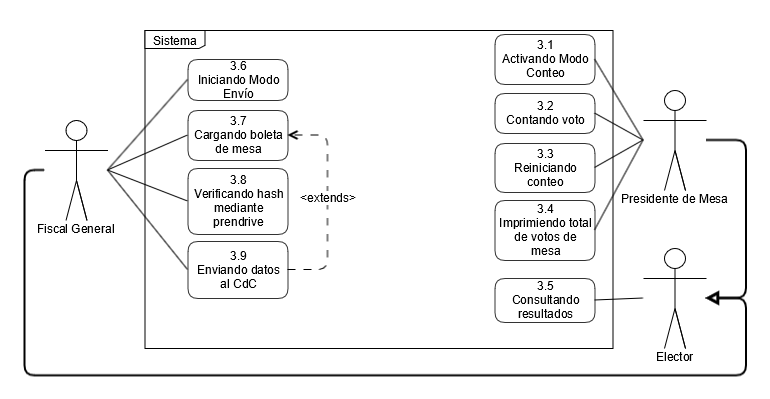
\includegraphics[scale=0.5]{imagenes/CU/casosdeusoconteo}
%\captionof{figure}{Diagrama de actividad}
\end{figure}			

A continuación presentaremos los detalles de casos de uso, estos sirven para profundizar el proceso de conteo y de fiscalización.


\textbf{Caso de uso: 3.1 - Activando modo conteo}

\textbf{Actor:} Presidente de mesa

\textbf{Pre:} Es el día de las elecciones, y se cerró la mesa del presidente.

\textbf{Post:} La máquina de sufragio se encuentra en modo conteo.

\begin{table}[h!]
	
 \begin{tabular}{|p{7.5cm} | p{7.5cm}|} 
 \hline
 \textbf{Curso normal} & \textbf{Curso Alternativo} \\
 \hline


1. El presidente de mesa se acerca a la máquina de sufragio asignada a su mesa junto con la urna y los fiscales. & \\
\hline

2. El presidente de mesa pone la máquina en modo conteo. & \\
\hline

3. El sistema carga inicializa una tabla interna donde carga todos los candidatos y les asigna 0 votos. Además, existe una columna para votos impugnados, y otra para votos en blanco. & \\
\hline

4. El presidente de mesa inserta una boleta vacía, donde se imprimirán los resultados totales de la mesa. El formato se explica más adelante. & \\
\hline

5. Fin de CU. & \\
\hline

\end{tabular}
\end{table}


\textbf{Caso de uso: 3.2 - Contando voto}

\textbf{Actor:} Presidente de mesa

\textbf{Pre:} Es el día de las elecciones y la máquina de sufragio se encuentra en modo conteo.

\textbf{Post:} La máquina de sufragio suma un voto más, algún candidato en cada categoría.

\newpage

\begin{table}[h!]
	
 \begin{tabular}{|p{7.5cm} | p{7.5cm}|} 
 \hline
 \textbf{Curso normal} & \textbf{Curso Alternativo} \\
 \hline


1. Si el presidente de mesa decidió impugnar el voto, selecciona la opción de impugnar voto. Ir al fin del caso de uso. & \\

\hline

2. Si no se impugnó el voto, se pasa la boleta por el lector de chip. & \\

\hline


3. La máquina lee el chip, y suma un voto en la tabla a los candidatos elegidos. & \\

\hline

4. La máquina muestra por pantalla los datos leídos. & \\

\hline

5. Fin de CU. & \\
\hline
\end{tabular}
\end{table}


\textbf{Caso de uso: 3.3 - Reiniciando conteo}

\textbf{Actor:} Presidente de mesa

\textbf{Pre:} Es el día de las elecciones y el fiscal general dio la orden de reiniciar el conteo.

\textbf{Post:} El conteo en la máquina de sufragio vuelve a 0.

\begin{table}[h!]
	
 \begin{tabular}{|p{7.5cm} | p{7.5cm}|} 
 \hline
 \textbf{Curso normal} & \textbf{Curso Alternativo} \\
 \hline


1. El presidente de mesa activa la opción de reiniciar el conteo. & \\
\hline

2. Se reinicia la tabla de conteo dentro de la máquina. & \\
\hline


3. Fin de CU. & \\
\hline
\end{tabular}
\end{table}


\textbf{Caso de uso: 3.4 - Imprimiendo total de votos}

\textbf{Actor:} Presidente de mesa

\textbf{Pre:} Es el día de las elecciones y se contaron todas las boletas de la urna.

\textbf{Post:} Se imprime en una boleta el total de los votos de la urna.

\begin{table}[h!]
	
 \begin{tabular}{|p{7.5cm} | p{7.5cm}|} 
 \hline
 \textbf{Curso normal} & \textbf{Curso Alternativo} \\
 \hline


1. El presidente de mesa elige la opción de imprimir resultados totales. & \\
\hline

2. La máquina de sufragio imprime el conteo total en la boleta. Los datos se imprimen tanto dentro del chip, como en tinta sobre la boleta. Sobre la boleta, se imprime una tabla que muestra todos los candidatos, y para cada uno la cantidad de votos que recibió. & \\
\hline

3. Fin de CU. & \\
\hline
\end{tabular}
\end{table}


\textbf{Caso de uso: 3.5 - Consultando resultados} 

\textbf{Actor:} Elector

\textbf{Pre:} Los resultados se encuentran publicados en la web.

\textbf{Post:} El elector conoce los resultados provisorios.

\begin{table}[h!]
	
 \begin{tabular}{|p{7.5cm} | p{7.5cm}|} 
 \hline
 \textbf{Curso normal} & \textbf{Curso Alternativo} \\
 \hline
 
1. El elector ingresa al sistema web público. & \\
\hline


2. Selecciona la opción de consulta de resultados. Una vez allí, conoce toda la información de los resultados. & \\
\hline


3. Fin de CU. & \\
\hline
\end{tabular}
\end{table}



\textbf{Caso de uso: 3.6 Iniciando modo envio}

\textbf{Actor:} Fiscal general

\textbf{Pre:} Es el día de las elecciones y el fiscal general posee la contraseña para activar el modo envío.

\textbf{Post:} La máquina se encuentra en modo envío.

\begin{table}[h!]
	
 \begin{tabular}{|p{7.5cm} | p{7.5cm}|} 
 \hline
 \textbf{Curso normal} & \textbf{Curso Alternativo} \\
 \hline

1. El fiscal general se acerca a la máquina de sufragio con conexión telefónica y la enciende. & \\
\hline

2. El fiscal general selecciona la opción de ingresar a modo envío. & \\
\hline

3. Luego, el sistema le pide la contraseña necesaria y él la ingresa. & \\
\hline

4. Se muestra mensaje de ingreso correcto. &
4.1. Si la contraseña no es correcta, se vuelve al paso 3. \\
\hline
5. Fin de CU. \\
\hline
\end{tabular}
\end{table}


\textbf{Caso de uso: 3.7 - Cargando boleta de mesa}

\textbf{Actor:} Fiscal general

\textbf{Pre:} Es el día de las elecciones una máquina de sufragio se encuentra en modo envío.

\textbf{Post:} La máquina de sufragio suma el resultado de una mesa más.

\begin{table}[h!]
	
 \begin{tabular}{|p{7.5cm} | p{7.5cm}|} 
 \hline
 \textbf{Curso normal} & \textbf{Curso Alternativo} \\
 \hline

1. El fiscal pasa la boleta por el lector de la máquina. Esta suma los resultados al conteo total y muestra en pantalla la información obtenida del chip. & \\
\hline

2. Si la boleta contada era la última, se extiende con CU 3.9 - Enviando datos al CdC. & \\
\hline

3. Fin de CU. & \\
\hline
\end{tabular}
\end{table}


\textbf{Caso de uso: 3.8 - Verificando hash mediante pendrive}


Es el mismo CU explicado en la etapa previa, el 2.1 - Verificando hash mediante pendrive


\textbf{Caso de uso: 3.9 - Enviando datos al CdC}

\textbf{Actor: }Fiscal general

\textbf{Pre:} Es el día de las elecciones y se cargaron todas las boletas de mesa.

\textbf{Post:} Se envió la información total de la escuela al CdC y ahora se encuentra guardada en el sistema.

\newpage

\begin{table}[h!]
	
 \begin{tabular}{|p{7.5cm} | p{7.5cm}|} 
 \hline
 \textbf{Curso normal} & \textbf{Curso Alternativo} \\
 \hline

1. El fiscal general elige la opción de enviar los resultados al Centro de Cómputos.  & \\
\hline

2. La máquina le pide que ingrese la contraseña única (la segunda contraseña que el fiscal General posee). & \\
\hline

3. El fiscal general la ingresa y selecciona “Enviar”. & \\
\hline

4. La máquina encripta el total de votos con la contraseña ingresada. & \\
\hline

5. La máquina envía los datos a través del enlace telefónico. & \\
\hline

6. El sistema en el CdC recibe la información y verifica que la encriptación se haya realizado con una contraseña válida. & \\
\hline

7. El sistema desencripta la información, y la almacena internamente para luego poder calcular los ganadores. & \\

\hline

8. Fin de CU. & \\
\hline
\end{tabular}
\end{table}
